\chapter{Quantum Metrology under Noise}
\label{ch:noise_analysis}

This chapter asks: if an $N$-qubit probe encodes the transverse field $h_x$, how much information about $h_x$ remains when an observer can access only $n$ qubits?  The observer's state is obtained by discarding the rest of the probe.

The central issue is \emph{local metrology}.  Quantum Fisher information (QFI) measures how rapidly a parameterized quantum state changes when $h_x$ changes: more local QFI means that, in principle, measurements on $S$ can estimate $h_x$ more precisely.  We are interested in how much QFI is lost by restricted access, and whether the answer depends on \emph{how the full probe was prepared} before $E$ was discarded.

The calculations follow Chapter~\ref{ch:methods}.  We evaluate QFI using the formalism of Chapter~\ref{ch:MathBackground}, and use the finite-displacement fidelity quantities from Section~\ref{sec:bounds} as complementary diagnostics.  The preparation history matters: a ground state, a globally Gibbs-prepared state, and a depolarized state can all give mixed states on $S$, but they are not the same physical experiment.

\begin{remark}[Chapter Summary]
    For the finite TFIM geometries, field windows, and state families studied here, retaining more qubits leaves more local QFI.  Depolarization provides a simple baseline and lowers local QFI monotonically in the sampled sweep.  In selected regimes, global Gibbs preparation leaves more local QFI than the reduced ground-state family.  This does not mean that a fixed thermal-noise channel increases QFI, nor does it establish a universal scaling law or a general benefit of temperature.
\end{remark}
% ==============================================================================
\section{The Problem and the Three Preparations}
\label{sec:noise_state_families}
% ==============================================================================
\subsection{Accessible and inaccessible qubits}

Let $S$ denote the accessible $n$-qubit subsystem and $E$ the inaccessible complement of $N-n$ qubits\footnote{In the standard quantum-information notation used here, $S$ denotes the system or subsystem of interest and $E$ its environment, the inaccessible complement.}.  The parameter $h_x$ serves as the estimation parameter $\theta$ of Chapters~\ref{ch:MathBackground} and~\ref{ch:methods}.  In all scenarios, restricted access is modeled by taking the partial trace $\operatorname{Tr}_E$ over $E$.  Here, \emph{local} means that only the subsystem $S$ is accessible; it does not restrict the observer to product measurements on the qubits within $S$.

The common open-chain Hamiltonian, and the backbone of every geometry used in studies, is the $N$-qubit TFIM defined in Eq.~\eqref{eq:tfim_hamiltonian}, with nearest-neighbor $ZZ$ coupling and a transverse field along $X$ (reported here for clarity).
\begin{equation}
    H_N(h_x)=-J\sum_{i=0}^{N-2}Z_iZ_{i+1}-h_x\sum_{i=0}^{N-1}X_i.
    \label{eq:noise_tfim_hamiltonian}
\end{equation}
In each numerical subsection, $H_N(h_x)$ denotes the finite-chain Hamiltonian for the geometry stated there. The numerical results use $J=1$, so that the phase transition occurs around $h_x\approx 1$ (we will see that it is typically before due to finite-size of the chain).

\begin{infobox}{What is being compared}
    Within each comparison, every branch starts from the same parameter-dependent TFIM Hamiltonian $H_N(h_x)$ and retains the same subsystem $S$.  What changes is how the full probe is prepared before the partial trace:
    \begin{enumerate}
        \item \textbf{Ground-state baseline.}  Prepare the full probe in its ground state and trace out $E$.  The resulting reduced state of $S$ can already be mixed, because $S$ and $E$ may be entangled.
        \item \textbf{Depolarizing control.}  Prepare the ground state, apply a fixed depolarizing channel to the full probe, and then trace out $E$.  This is the only fixed, parameter-independent noise channel considered here.
        \item \textbf{Thermal family.}  Prepare the full probe in the Gibbs state at fixed inverse temperature $\beta$, and then trace out $E$.  This is a distinct parameter-dependent preparation family, not a fixed channel applied to the ground-state family.
    \end{enumerate}
    An important note is that the main comparison is not ``the same state with two kinds of noise.''  It is a comparison of three reduced states produced by three distinct physical histories.  Secondly, the traced-out subsystem $E$ is not the external bath used to prepare a Gibbs state, it is simply the finite portion of the probe to which the observer has no local access.
\end{infobox}

\begin{definition}[Prepared and reduced state families]
    The ground-state reference, depolarized, and thermal families are
    \begin{align}
        \rho_{\mathrm{G},N}(h_x)
         & \coloneqq |\psi_0(h_x)\rangle\langle\psi_0(h_x)|,              &
        \rho_{\mathrm{G},S}(h_x)
         & \coloneqq \operatorname{Tr}_E[\rho_{\mathrm{G},N}(h_x)]          \\
        \rho_{\mathrm{dep},N}(h_x;P)
         & \coloneqq \Lambda^{(N)}_P[\rho_{\mathrm{G},N}(h_x)],           &
        \rho_{\mathrm{dep},S}(h_x;P)
         & \coloneqq \operatorname{Tr}_E[\rho_{\mathrm{dep},N}(h_x;P)]      \\
        \rho_{\mathrm{th},N}(h_x;\beta)
         & \coloneqq \frac{\exp[-\beta H_N(h_x)]}{Z(h_x,\beta)},          &
        \rho_{\mathrm{th},S}(h_x;\beta)
         & \coloneqq \operatorname{Tr}_E[\rho_{\mathrm{th},N}(h_x;\beta)]   \\
        \text{Where: } Z(h_x,\beta)
         & \coloneqq \operatorname{Tr}[\exp[-\beta H_N(h_x)]]
        \label{eq:noise_state_families}
    \end{align}
    Here $\beta$ is the inverse temperature of the Gibbs preparation: larger $\beta$ means a colder Gibbs state.  When the ground state is nondegenerate, the Gibbs family approaches the ground-state reference as $\beta\to\infty$. At a degeneracy, it instead approaches the normalized projector onto the ground-state subspace. The notation follows    $\rho_{\text{family}, \text{ system\_size}}$.
\end{definition}


The full-system depolarizing channel used in this chapter is
\begin{equation}
    \Lambda_P^{(N)}(\rho)
    =(1-P)\rho+P\frac{\mathbb{I}_{2^N}}{2^N},
    \qquad 0\leq P\leq1.
    \label{eq:full_depolarizing_channel}
\end{equation}
It replaces the input by the maximally mixed $N$-qubit state with probability $P$. Since depolarization is applied before the partial trace,
\begin{equation}
    \rho_{\mathrm{dep},S}(h_x;P)
    =(1-P)\rho_{\mathrm{G},S}(h_x)
    +P\frac{\mathbb{I}_{2^n}}{2^n}.
    \label{eq:reduced_depolarizing_state}
\end{equation}

The three primary local states are $\rho_{\mathrm{G},S}$, $\rho_{\mathrm{dep},S}$, and $\rho_{\mathrm{th},S}$.  They have the same accessible Hilbert-space dimension, but not the same spectrum or dependence on $h_x$.  Each full-system curve is a reference ceiling for the reduced state in the corresponding preparation family. The physical question is always what an observer can learn while having access only to $S$.

A diagrammatic summary is:

\[
    h_x\longrightarrow H_N(h_x)\longrightarrow |\psi_0(h_x)\rangle
    \longrightarrow \rho_{\mathrm{G},N}(h_x)
    \xrightarrow{\operatorname{Tr}_E}\rho_{\mathrm{G},S}(h_x)
    \longrightarrow \text{Local QFI}.
\]
There is no external noise map. The subsystem is mixed because it is correlated with the discarded degrees of freedom. We also picture a category theory graphical calculus version of the channels, based on \cite{wood2015graphical}.


\begin{figure}[H]
    \centering
    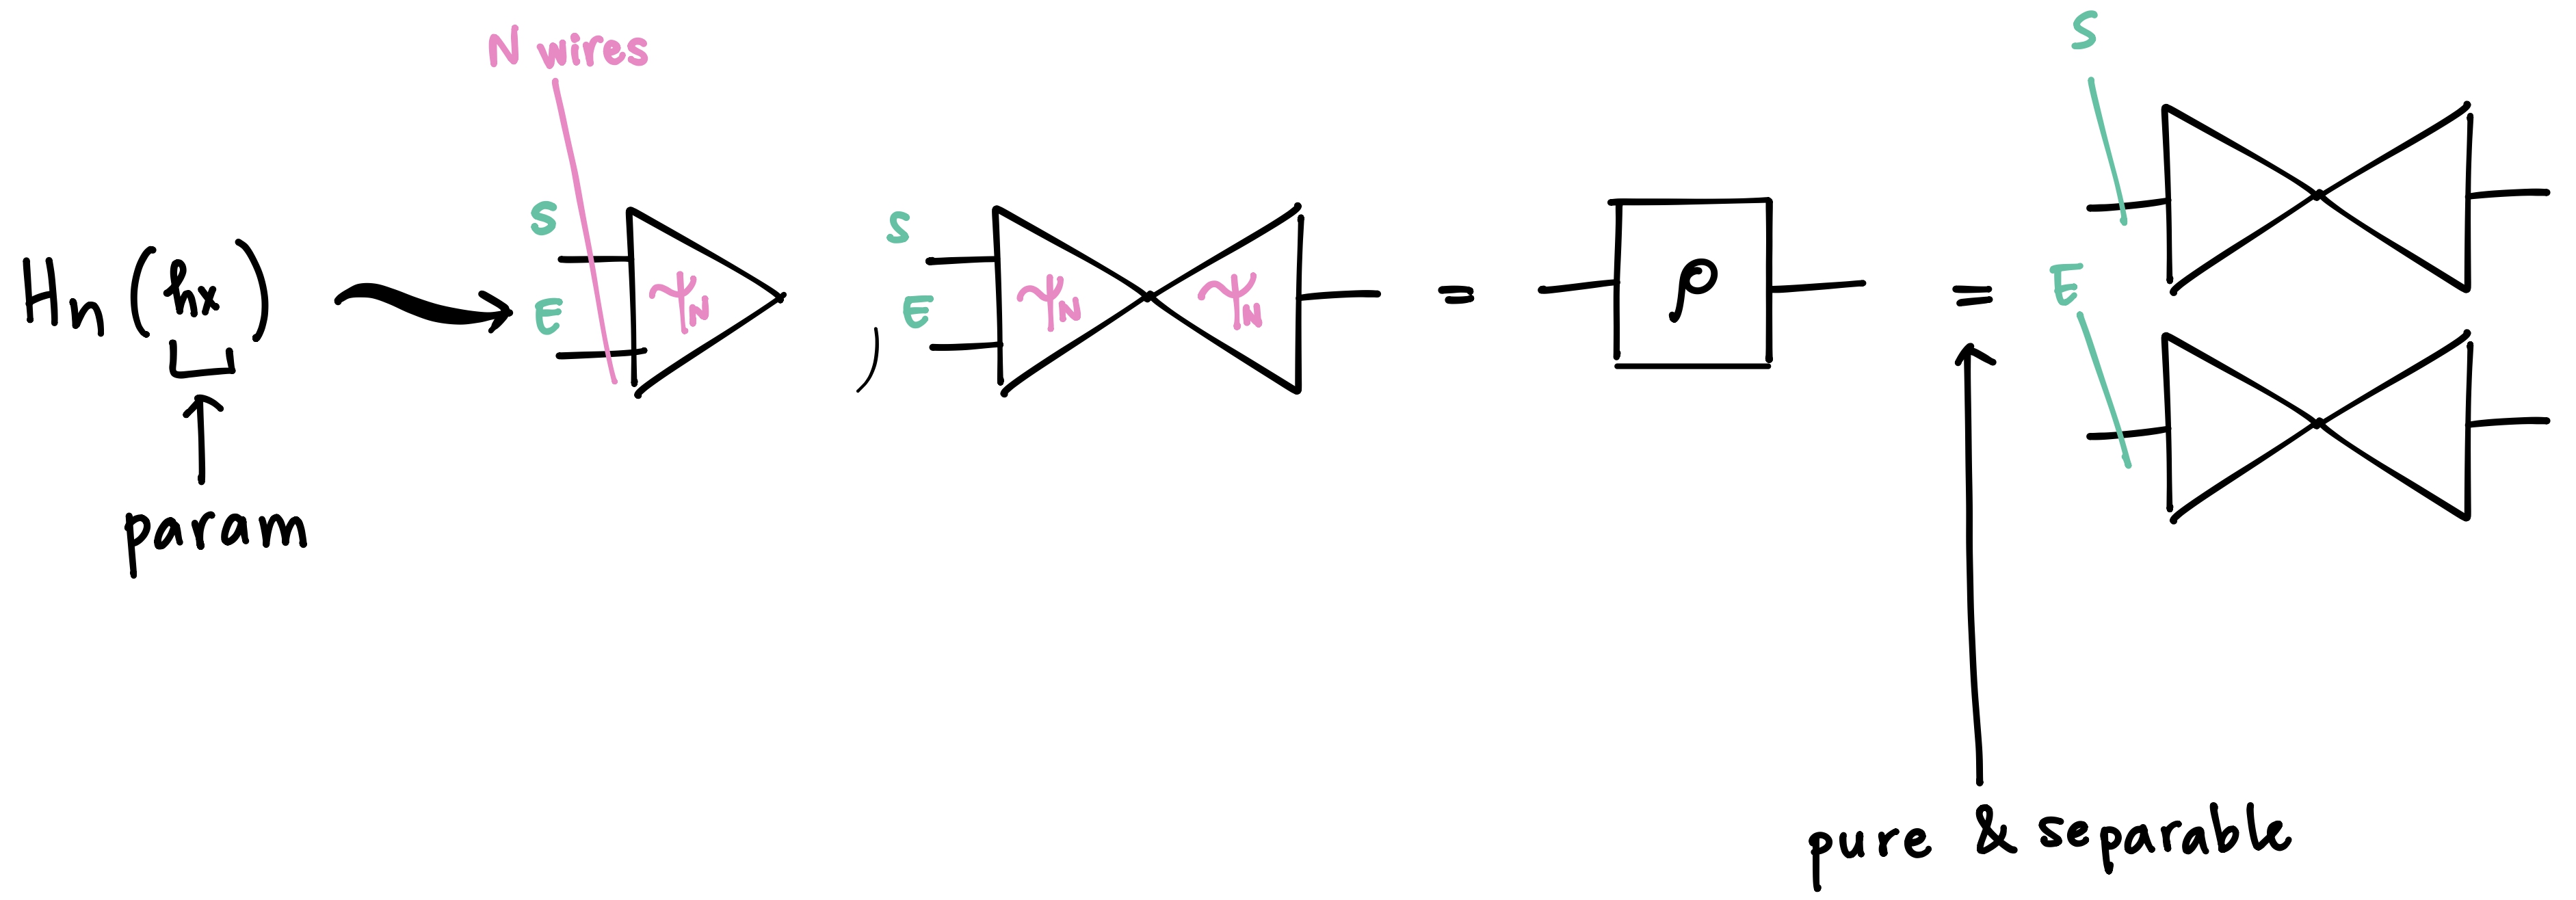
\includegraphics[width=\textwidth]{figures/diagrams/diagram_encoding_hamiltonian.jpg}
    \caption{Diagrammatic summary of how the parameter $h_x$ is encoded in the Hamiltonian, the state and the density matrix are created, in this initial phase the system is still separable.}
    \label{fig:diagram_encoding_hamiltonian}
\end{figure}


\begin{figure}[H]
    \centering
    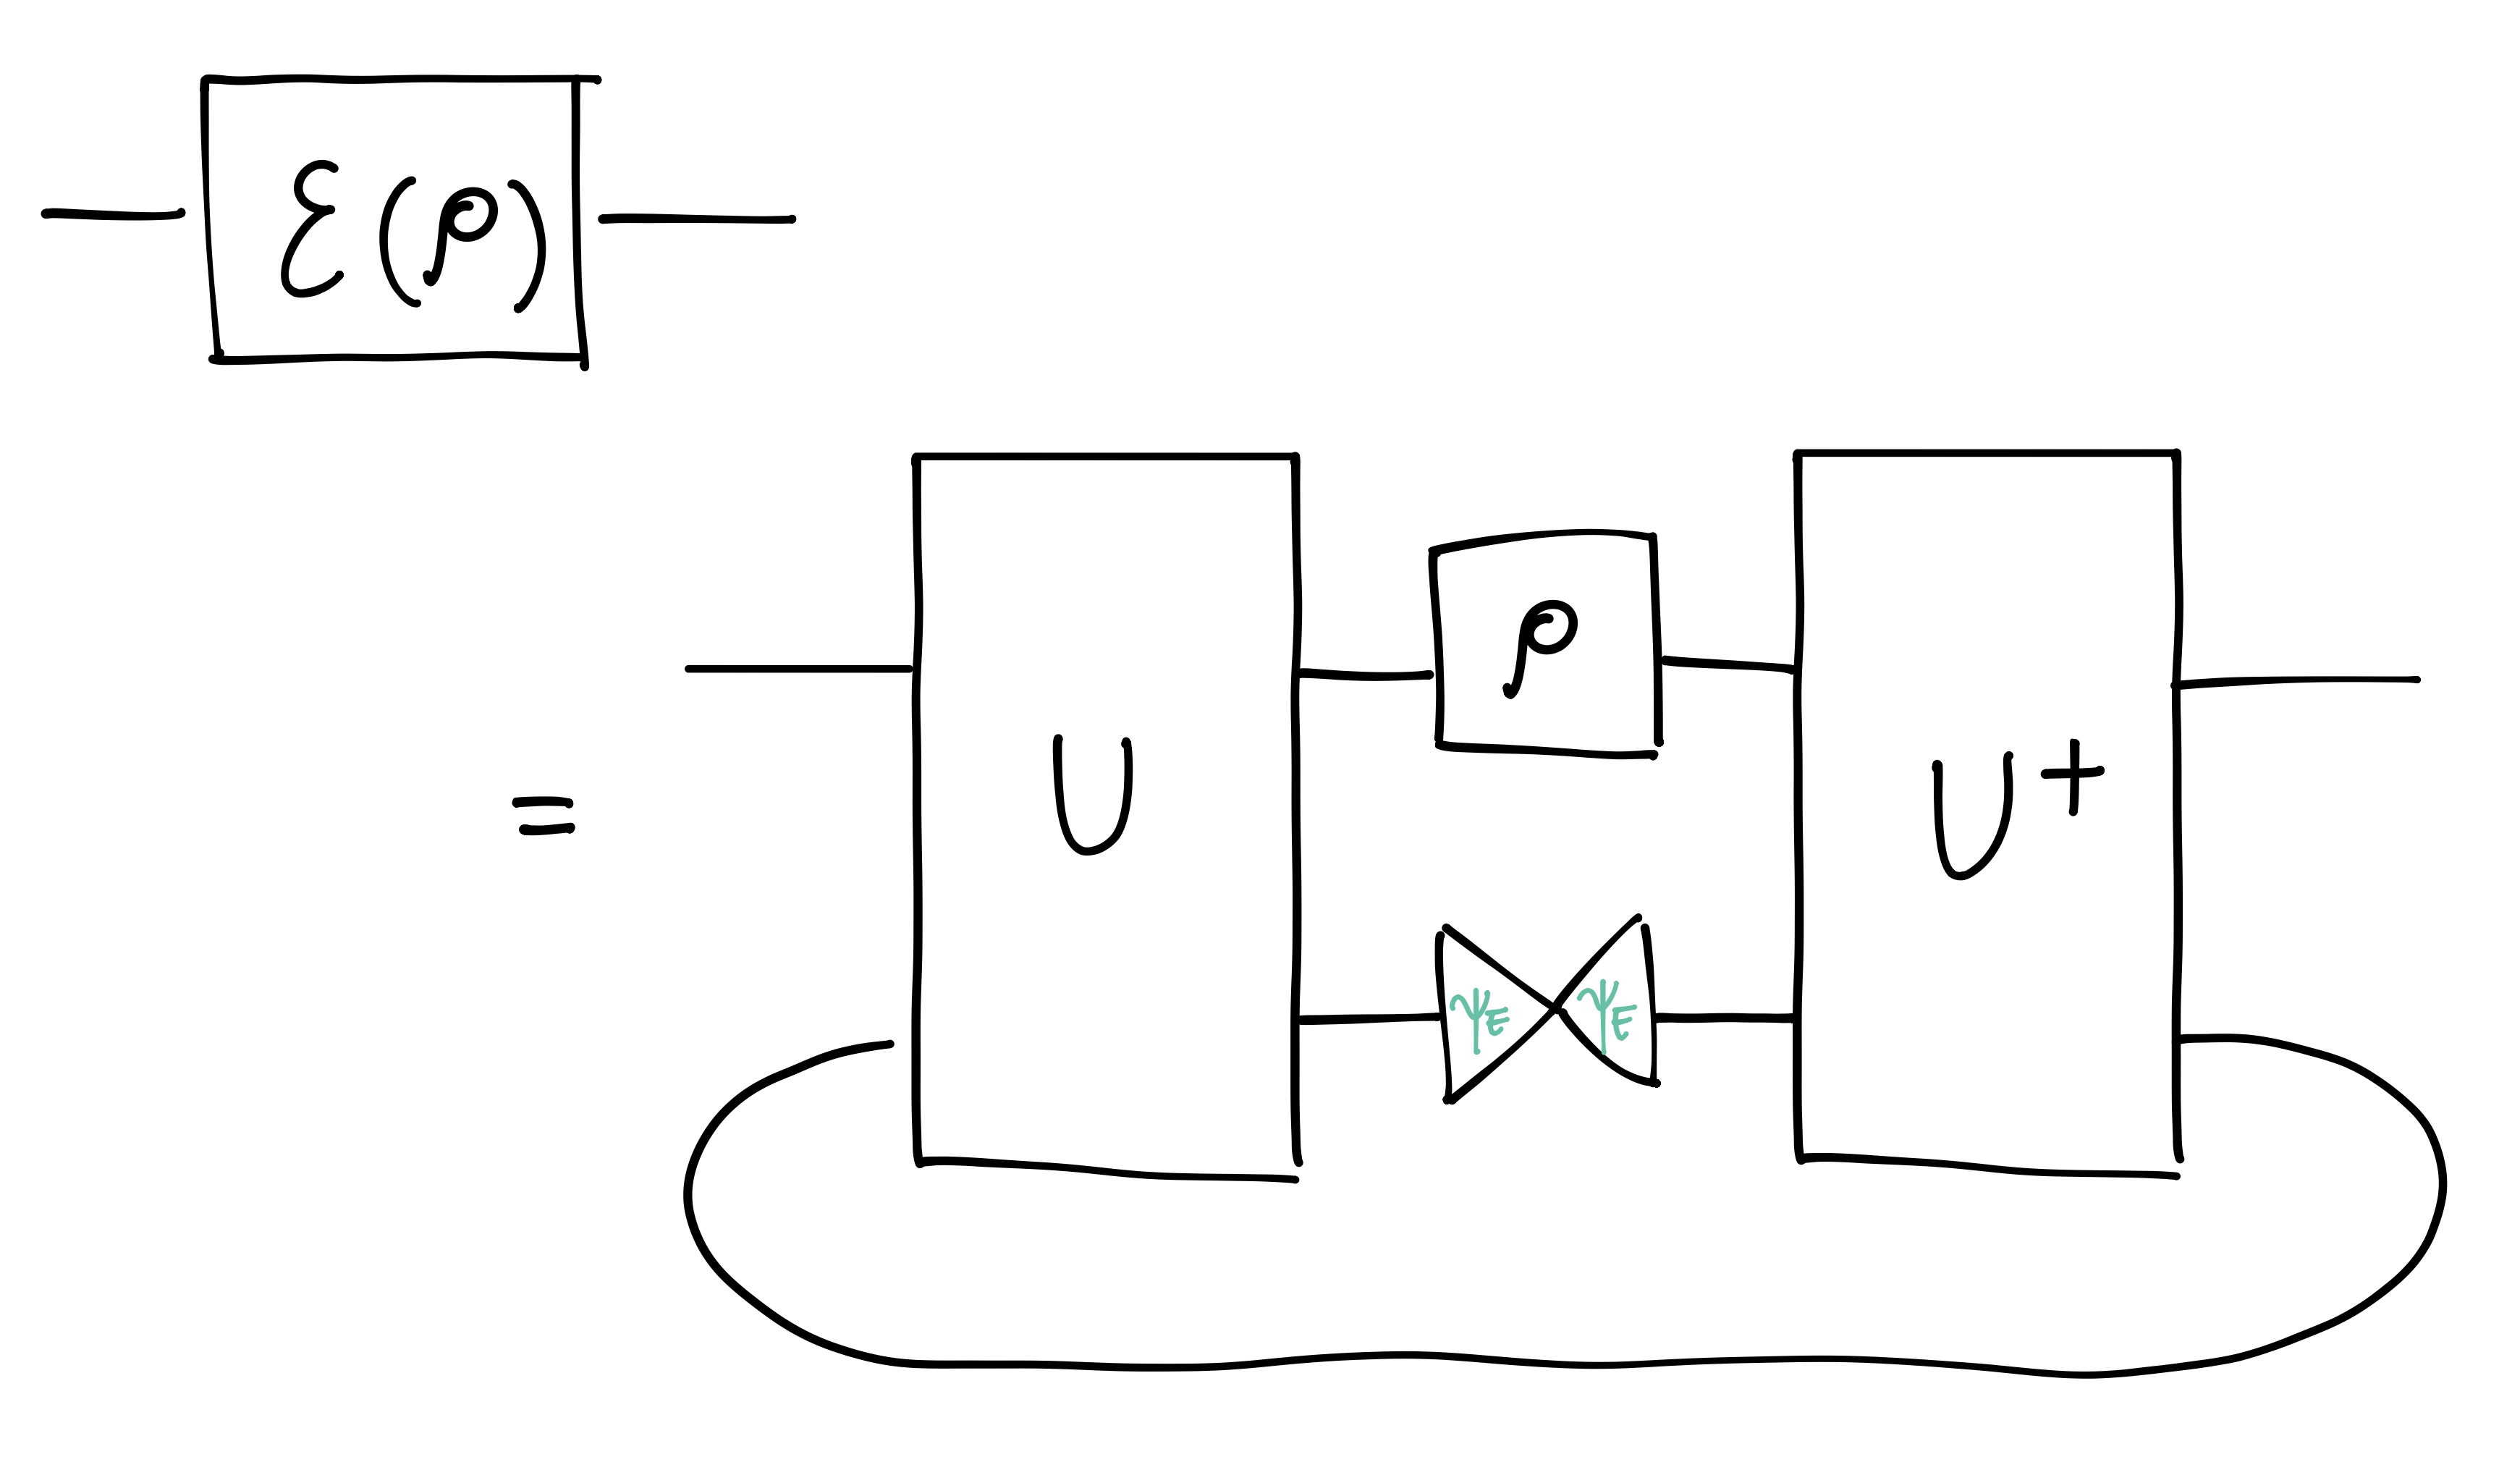
\includegraphics[width=0.6\textwidth]{figures/diagrams/diagram_stinespring_to_kraus.jpg}
    \caption{Stinespring system representation.  The system $S$ is the accessible subsystem, while $E$ is the inaccessible complement.  The Stinespring representation is useful because we can consider a unitary $U$ acting on the state state and on the environment. The partial trace over $E$, represented as a closed loop, connecting the wires, produces the reduced state of $S$. It is equivalent to the channel representation of the same process, which is obtained by applying the Kraus operators $K_i$ to the state of $S$ (See. the graphical proof in Fig.~\ref{fig:diagram_stinespring_to_kraus_extended_proof}).}
    \label{fig:diagram_stinespring_evolution}
\end{figure}

The depolarizing channel is parameter independent when $P$ is fixed, it can also be described clearly with a Choi, Stinespring, or Kraus representation.
\[
    \rho_{\mathrm{G},N}(h_x)
    \xrightarrow{\Lambda_P^{(N)}}\rho_{\mathrm{dep},N}(h_x;P)
    \xrightarrow{\operatorname{Tr}_E}\rho_{\mathrm{dep},S}(h_x;P)
    \longrightarrow \text{local QFI}.
\]

\begin{figure}[htbp]
    \centering
    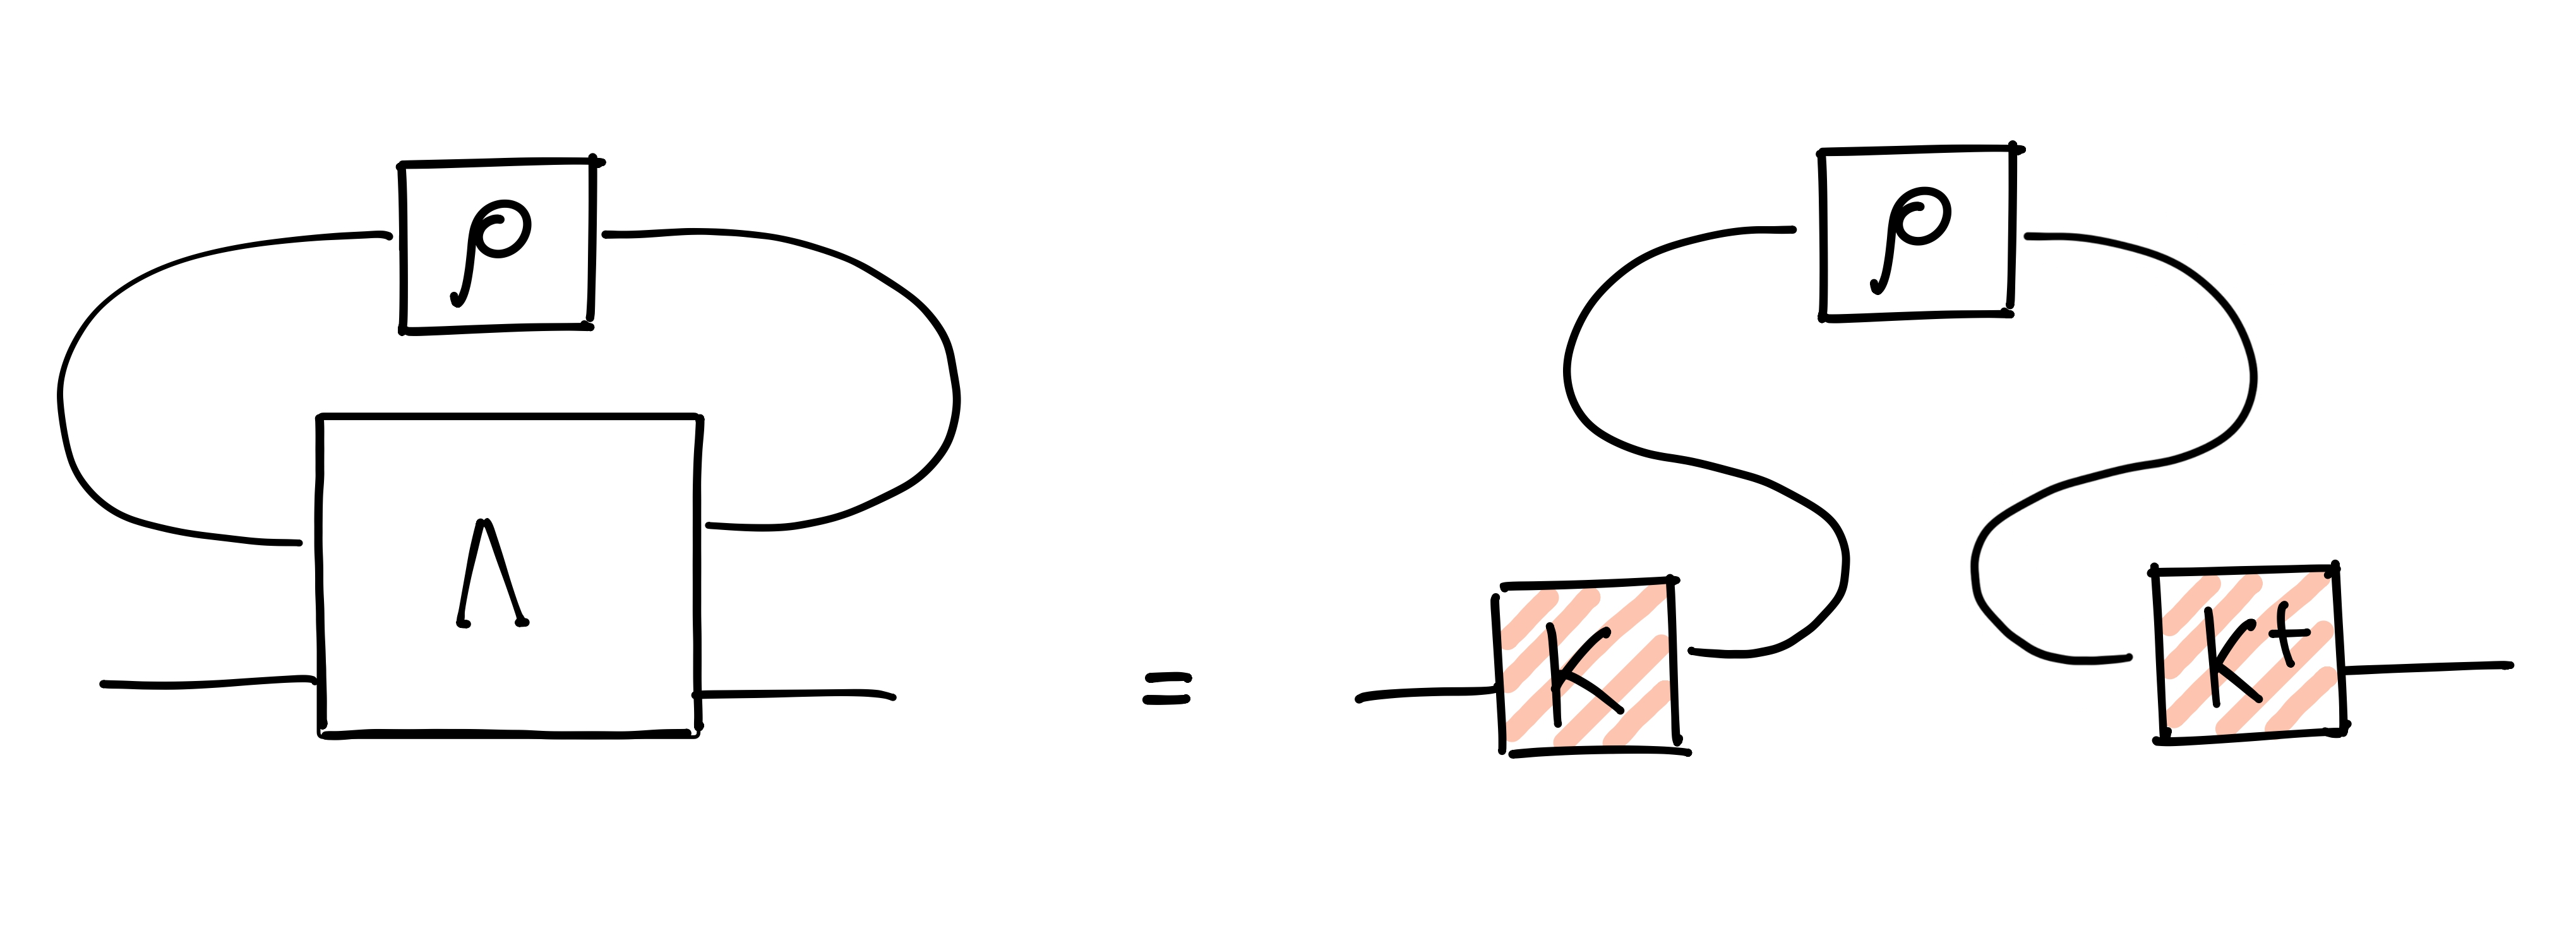
\includegraphics[width=0.7\textwidth]{figures/diagrams/diagram_Choi_to_kraus.jpg}
    \caption{Equivalence between the Choi representation and the Kraus representation.}
    \label{fig:diagram_Choi_to_kraus}
\end{figure}


Thermal branch has a different initialization,that both $H_N$ and the Gibbs state depend on $h_x$.This branch begins from a separately prepared Gibbs state.  It does not apply a thermal channel to $\rho_{\mathrm{G},N}$.
\[
    h_x\longrightarrow H_N(h_x)\longrightarrow\rho_{\mathrm{th},N}(h_x;\beta)
    \xrightarrow{\operatorname{Tr}_E}\rho_{\mathrm{th},S}(h_x;\beta)
    \longrightarrow \text{local QFI}.
\]



\begin{infobox}{Scope of the Thermal Model}
    The thermal branch does not model dynamical thermalization of the accessible subsystem by the discarded qubits. Instead, we assume that the full finite TFIM probe has been prepared in the Gibbs state
    \[
        \rho_{\mathrm{th},N}(h_x;\beta)
        =
        \frac{e^{-\beta H_N(h_x)}}{Z(h_x,\beta)}
    \]
    by an external, unmodelled equilibrium-preparation mechanism. We then restrict access to the subsystem $S$ by tracing out the complementary degrees of freedom $E$. So $E$ represents an inaccessible part of the prepared probe, not to be confused with the macroscopic thermal bath. In general,
    \[
        \operatorname{Tr}_E[\rho_{\mathrm{th},N}]
        \neq
        \frac{e^{-\beta H_S}}{\operatorname{Tr}[e^{-\beta H_S}]}
    \]
    because interactions across the $S$--$E$ boundary and their correlations remain encoded in the reduced state. Our model  studies the local metrological consequences of global thermal preparation, rather than a microscopic thermalization dynamics.
\end{infobox}


\subsection{Which comparisons are valid?}

This was a delicate point during our study, since the results can become counterintuitive.  For a fixed $P$, the depolarizing channel and the partial trace are parameter-independent channels.  QFI cannot increase under either operation, giving
\begin{equation}
    \mathcal{F}_Q[\rho_{\mathrm{dep},S}(h_x;P)]
    \leq \mathcal{F}_Q[\rho_{\mathrm{dep},N}(h_x;P)]
    \leq \mathcal{F}_Q[\rho_{\mathrm{G},N}(h_x)]
    \label{eq:depolarizing_data_processing}
\end{equation}
In the same way, restricted access cannot increase the QFI within the ground-state and thermal families:
\begin{equation}
    \mathcal{F}_Q[\rho_{\mathrm{G},S}(h_x)]
    \leq \mathcal{F}_Q[\rho_{\mathrm{G},N}(h_x)],
    \qquad
    \mathcal{F}_Q[\rho_{\mathrm{th},S}(h_x;\beta)]
    \leq \mathcal{F}_Q[\rho_{\mathrm{th},N}(h_x;\beta)].
    \label{eq:local_global_data_processing}
\end{equation}

These inequalities compare a full probe and a reduced probe \emph{within the same preparation family}, and are trivial. But they do not imply
\begin{equation}
    \mathcal{F}_Q[\rho_{\mathrm{th},S}(h_x;\beta)]
    \leq
    \mathcal{F}_Q[\rho_{\mathrm{G},S}(h_x)]
    \qquad
    \text{(not guaranteed)}
    \label{eq:no_cross_family_qfi_ordering}
\end{equation}
At fixed $\beta$, Gibbs preparation defines a different $h_x$-dependent family, not a parameter-independent channel applied to the ground state.  The thermal and reduced-ground-state QFIs therefore have no universal ordering.  A thermal--ground comparison is consistent with data processing provided that the thermal local QFI remains below that of its full thermal parent.

\subsection{Fixed controls and matched purity}

Most comparisons keep the physical preparation control fixed while sweeping
$h_x$. So the depolarizing probability $P$ is fixed for the depolarizing family,
and the inverse temperature $\beta$ is fixed for the Gibbs family.  This is
the setting that describes one preparation protocol operated across the field
scan.

A \emph{matched purity} regime is used as a separate diagnostic.  Writing
$\gamma(\rho)=\operatorname{Tr}(\rho^2)$, it chooses $P(h_x)$ and
$\beta(h_x)$ so that
\begin{equation}
    \gamma\!\left(\rho_{\mathrm{dep},S}(h_x;P(h_x))\right)
    =
    \gamma\!\left(\rho_{\mathrm{th},S}(h_x;\beta(h_x))\right)
    =
    \gamma_{\mathrm{target}}(h_x)
    \label{eq:purity_matching_cond}
\end{equation}
The target can be a number $\gamma_{\mathrm{target}} \in [\frac{1}{d},1]$, representing the purity of a reference reduced state. In this case d is the dimension of the system.  This asks a simple
question: if two local states are equally mixed according to their purity, do
they also have the same local QFI?  The matched-purity results are discussed
in Section~\ref{sec:project10_peak_purity}.

\begin{infobox}{Why matched-purity QFI requires care}
    In a field-by-field purity match, $P$ and $\beta$ change with $h_x$.
    The QFI must follow that chosen path through state space.  If
    $\rho$ depends on a control $\lambda(h_x)$, then
    \begin{equation}
        \frac{\mathrm{d}\rho}{\mathrm{d}h_x}
        =
        \frac{\partial\rho}{\partial h_x}
        +
        \frac{\partial\rho}{\partial\lambda}
        \frac{\mathrm{d}\lambda}{\mathrm{d}h_x}
        \label{eq:matched_path_total_derivative}
    \end{equation}
    Here $\lambda$ is $P$ or $\beta$.  This is different from the
    fixed-control calculations, where the second term is absent.  The
    field-by-field match is therefore useful for testing the role of purity,
    but it is not the response of one fixed noisy device.
\end{infobox}


% ==============================================================================
\section{What Is Calculated and Compared}
\label{sec:noise_observables}
% ==============================================================================

For each $h_x$, the calculation constructs a state family, discards $E$, and asks how strongly the resulting local state changes.  We also evaluate fidelity quantities from $\rho(h_x)$ and $\rho(h_x+\delta h_x)$, because these are the quantities accessible to a truncation-based metrology protocol.  The finite-displacement functional is defined in Eq.~\eqref{eq:qfi_difference_quotient}. For the exact SLD benchmarks reported here, the density-matrix derivatives are evaluated analytically. The matched-purity families additionally include the chain-rule contribution in Eq.~\eqref{eq:matched_path_total_derivative}. The central-difference formula in Eq.~\eqref{eq:central_difference} is a fallback for cases in which an analytical derivative is unavailable, and its derivative step must not be confused with the forward displacement $\delta h_x$ used by TQFI.

\begin{remark}[Exact QFI and TQFI serve different purposes]
    Exact SLD QFI is the local, infinitesimal benchmark that supports the physical claims in this chapter. TQFI is a finite-displacement, truncation-aware diagnostic. At nonzero $\delta h_x$, its lower and upper endpoints bound the finite-displacement functional $\mathcal I_{\delta}$, not the exact SLD QFI. A finite-displacement lower TQFI value can therefore exceed the exact SLD value without violating the TQFI inequality. Exact SLD values may be compared when the physical families agree, but raw TQFI magnitudes should not be compared across projects without accounting for different displacement and truncation settings.
\end{remark}

The numerical settings relevant to these comparisons are summarized below:
\begin{table}[htbp]
    \centering
    \caption{Field grids and finite-displacement settings. The truncation rank $m$ applies only to TQFI calculations. SSQFI does not use spectral truncation.}
    \label{tab:noise_numerical_settings}
    \begin{tabular}{l c c c}
        \toprule
        Study                                & Field grid                 & $\delta h_x$ & $m$ \\
        \midrule
        Restricted-access study (Project~1)  & $50$ points on $[0.1,2.1]$ & $0.1$        & $2$ \\
        Gibbs-temperature study (Project~7)  & $60$ points on $[0.1,2.5]$ & $0.1$        & $2$ \\
        Three-family comparison (Project~9)  & $60$ points on $[0.1,2.5]$ & $0.05$       & $3$ \\
        Fixed purity comparison (Project~10) & $60$ points on $[0.1,2.5]$ & ---          & --- \\
        \bottomrule
    \end{tabular}
\end{table}
For the one-qubit Project~9 subsystem, $m$ is capped at the Hilbert-space dimension, so $m=2$. Where a result is explicitly described as a \emph{refined maximum}, a bounded continuous optimization is performed within the bracket containing the coarse-grid maximum to find the precise maximum. Otherwise the reported maximum is over the stated field grid.

The results are presented in three steps.  First, we establish the loss caused by restricting access to part of the probe.  Then we examine the thermal family and its temperature dependence.  Finally, we compare the three preparation histories at fixed accessible size.
% ==============================================================================
\section{Restricted Access Alone}
\label{sec:project1_noise}
% ==============================================================================

The first calculation is the reference case.  The full probe is prepared in its ground state, no external noise channel is applied, and only then is $E$ discarded.  This isolates the information loss caused by restricting access to $S$.

\subsection{Changing total and accessible size}

The open-chain sequence $(N,n)=(4,2),(6,4),(8,6)$ changes both total size and accessible fraction.

\begin{table}[htbp]
    \centering
    \caption{Open-chain scaling sequence with $n=N-2$. Values and locations are using \emph{refined maximum}.}
    \label{tab:project1_size_sequence}
    \begin{tabularx}{\textwidth}{
            c
            >{\centering\arraybackslash}X
            >{\centering\arraybackslash}X
            >{\centering\arraybackslash}X
            >{\centering\arraybackslash}X
            >{\centering\arraybackslash}X
        }
        \toprule
        \thead{$(N,n)$} &
        \thead{Peak local                \\ SLD} &
        \thead{Peak full                 \\ SLD} &
        \thead{Local /                   \\ full} &
        \thead{Peak                      \\ lower TQFI } &
        \thead{Peak                      \\ sub QFI} \\
        \midrule
        $(4,2)$         & \thead{$2.859$ \\at $0.508$ } & \thead{$4.395$ \\at $0.435$ } & $0.651$ & $1.969$ & $1.419$ \\
        $(6,4)$         & \thead{$5.935$ \\at $0.646$ } & \thead{$6.788$ \\at $0.620$ } & $0.874$ & $3.164$ & $1.413$ \\
        $(8,6)$         & \thead{$9.517$ \\at $0.730$ } & \thead{$10.068$ \\at $0.719$} & $0.945$ & $4.440$ & $1.330$ \\
        \bottomrule
    \end{tabularx}
\end{table}

% \noindent\emph{Peak-position note.} The original field grid has a spacing of about $0.041$, so its maxima cannot resolve nearby continuous peak locations. The values in Table~\ref{tab:project1_size_sequence} instead result from bounded optimization inside the grid bracket containing each coarse maximum. For example, the refined $N=6$, $n=4$ local and full peaks are at $h_x^\star=0.64606$ and $0.61979$, respectively, although both fall in the same coarse-grid bin.

\begin{figure}[H]%[htbp]
    \centering
    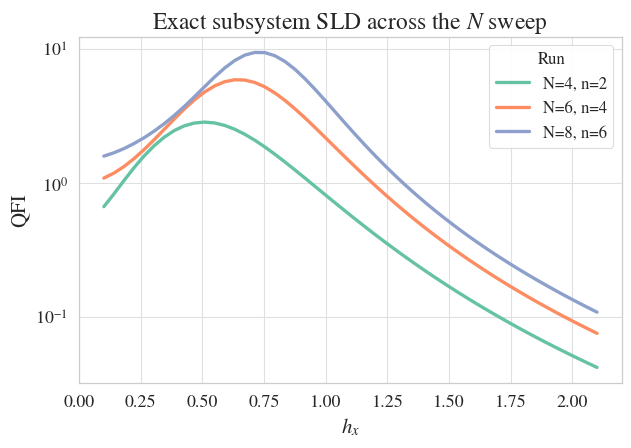
\includegraphics[width=0.8\textwidth]{figures/noise/project1/proj1_fig_1_1.png}
    \caption{Exact local SLD QFI and finite-displacement fidelity diagnostics for the three open-chain size pairs in Table~\ref{tab:project1_size_sequence}.}
    \label{fig:project1_fig_1_1}
\end{figure}


The local peak rises strongly, while the retained fraction of the full peak increases from about $65\%$ to $94.5\%$. Intuitively, the inaccessible complement remains two qubits while the accessible subsystem grows. Partial trace is the only loss mechanism in this baseline. As the total size increases, the full finite-size peaks move towards the thermodynamic critical value $h_x/J=1$.

\subsection{Retaining more qubits at fixed total size}

\begin{table}[H]%[htbp]
    \centering
    \caption{Recovery of the full-system peak as the accessible subsystem grows at fixed open-chain size $N=8$. The full-system maximum is $10.068$ at $h_x^\star=0.719$. See Figure~\ref{fig:project1_fig_1_3}.}
    \label{tab:project1_subsystem_sequence}
    \begin{tabular}{c c c c}
        \toprule
        $n$ & Peak local SLD QFI & $h_{x,\mathrm{local}}^\star$ & Fraction of full SLD peak \\
        \midrule
        $2$ & $3.252$            & $0.784$                      & $0.323$                   \\
        $3$ & $5.170$            & $0.767$                      & $0.514$                   \\
        $4$ & $6.933$            & $0.756$                      & $0.689$                   \\
        $5$ & $8.410$            & $0.741$                      & $0.835$                   \\
        $6$ & $9.517$            & $0.730$                      & $0.945$                   \\
        $7$ & $10.068$           & $0.719$                      & $1.000$                   \\
        \bottomrule
    \end{tabular}
\end{table}

It is important to study how the approximated local peaks positions are situated with respect to the full-system ones, since that is the best, real operative range for the metrology.
Retaining more qubits gives rapid, monotonic recovery of the critical response.  For a fixed $N=8$, a bounded continuous optimization of the exact SLD QFI around each coarse-grid maximum shows that the local peak position converges monotonically to the full-system finite-size peak as $n$ increases.  When only one qubit is traced out, the two peak positions coincide at $h_x^\star=0.71897$.  The relevant reference is this finite-$N$ pseudo-critical peak, rather than the thermodynamic value $h_x/J=1$.

\begin{figure}[H]
    \centering
    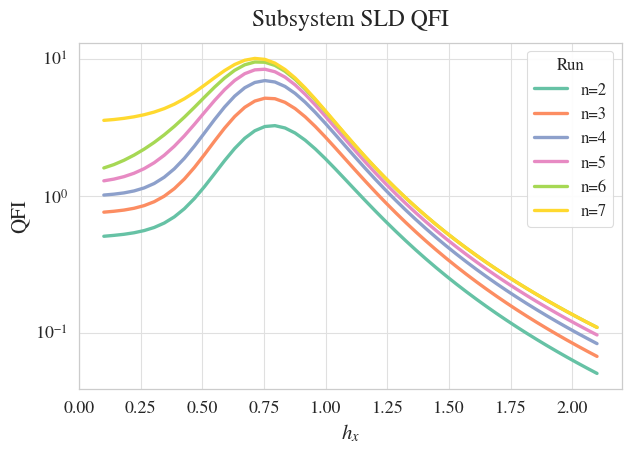
\includegraphics[width=0.55\textwidth, valign=c]{figures/noise/project1/subsystem_SLD_varying_n_fixing_N8.png}
    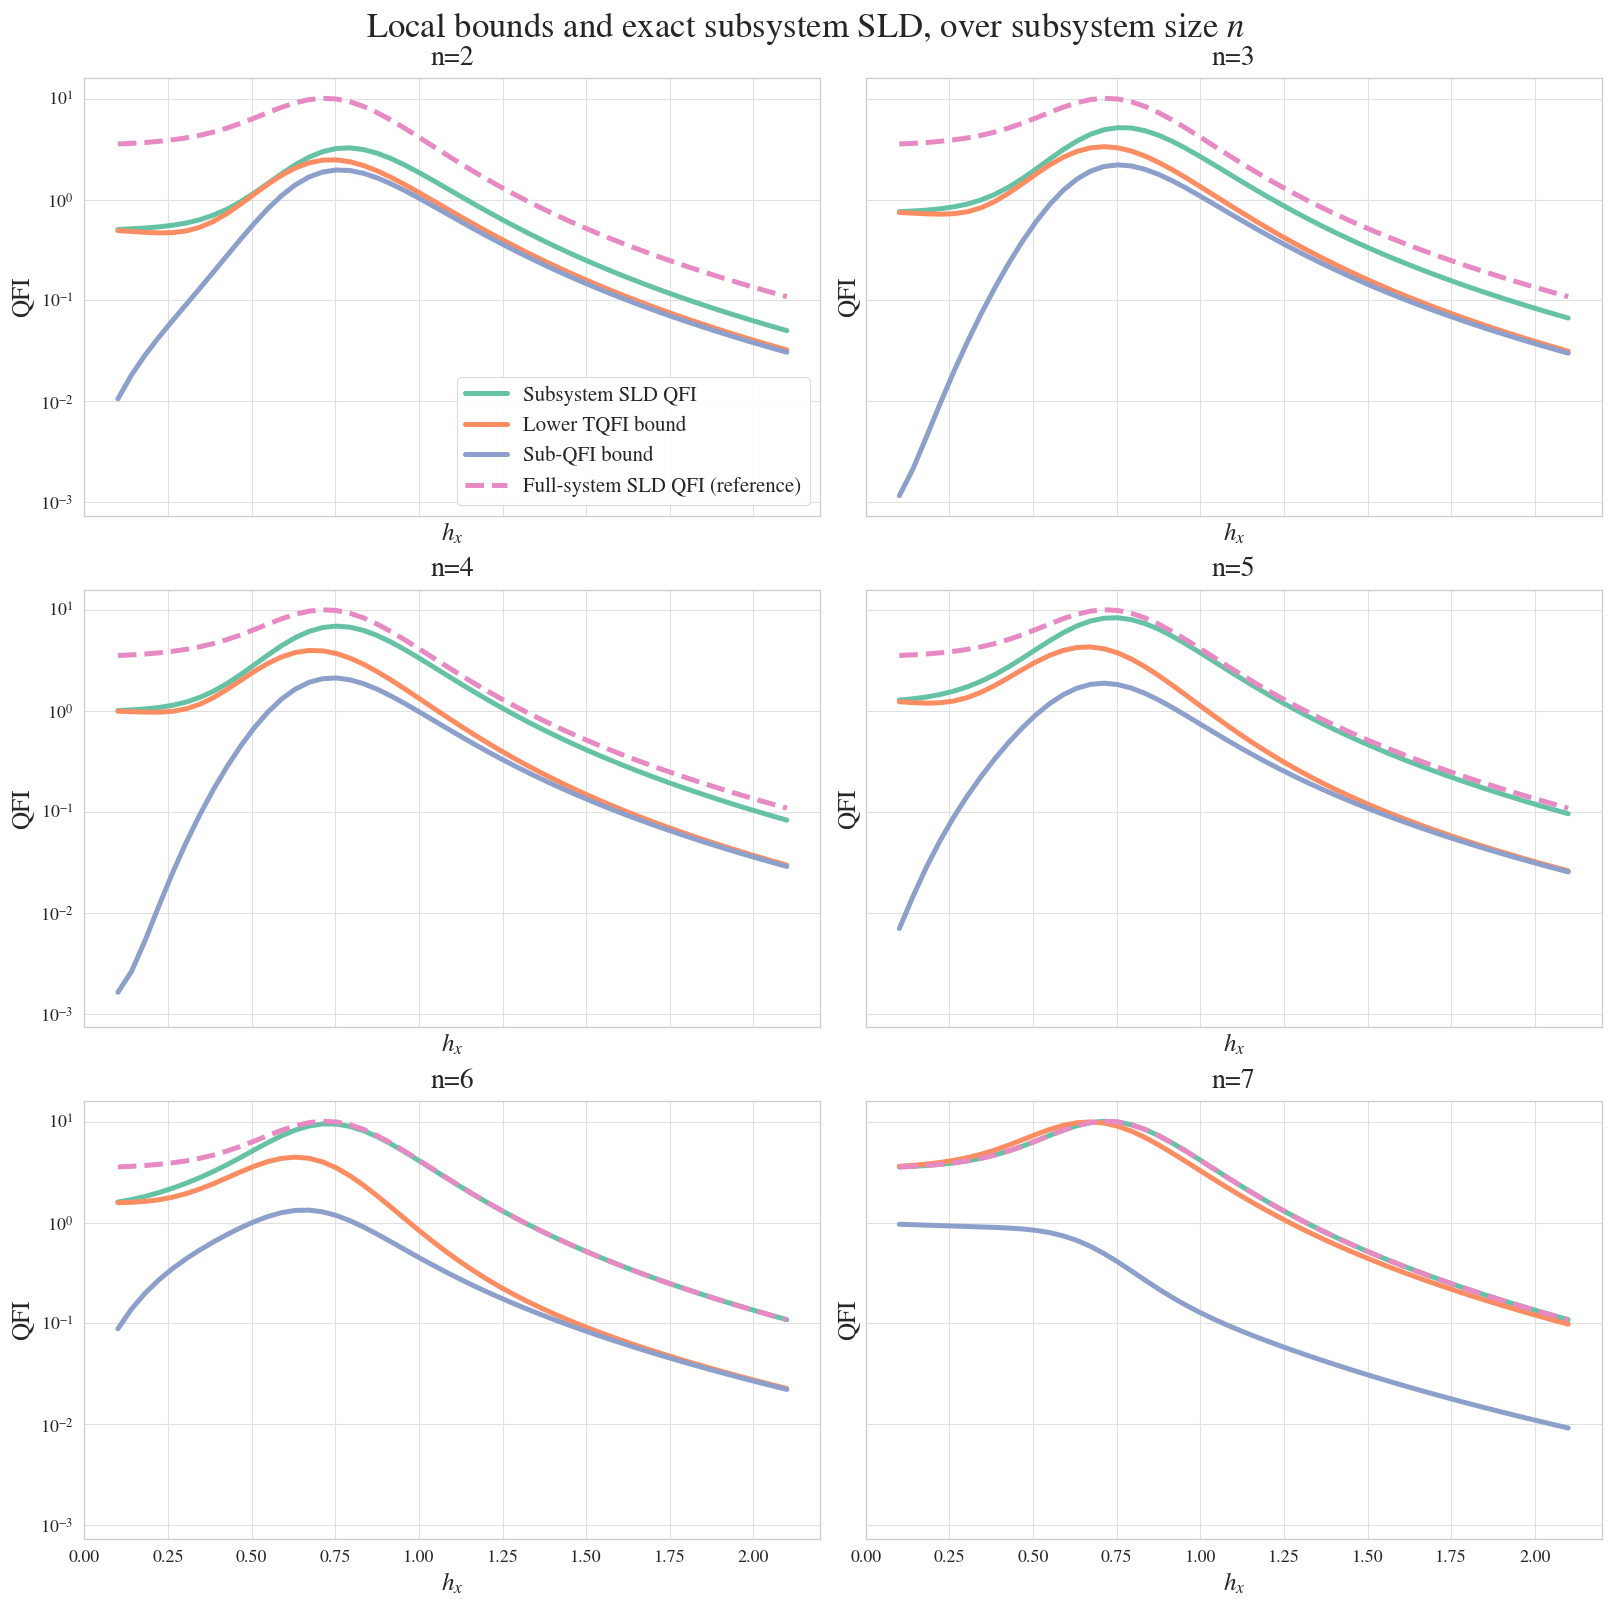
\includegraphics[width=0.80\textwidth, valign=c]{figures/noise/project1/local_bounds_and_exact_over_n_subsystem.png}
    \caption{Recovery of the exact local SLD QFI and finite-displacement diagnostics as the accessible subsystem size $n$ increases at fixed $N=8$.}
    \label{fig:project1_fig_1_3}
\end{figure}


\begin{figure}[H]%[htbp]
    \centering
    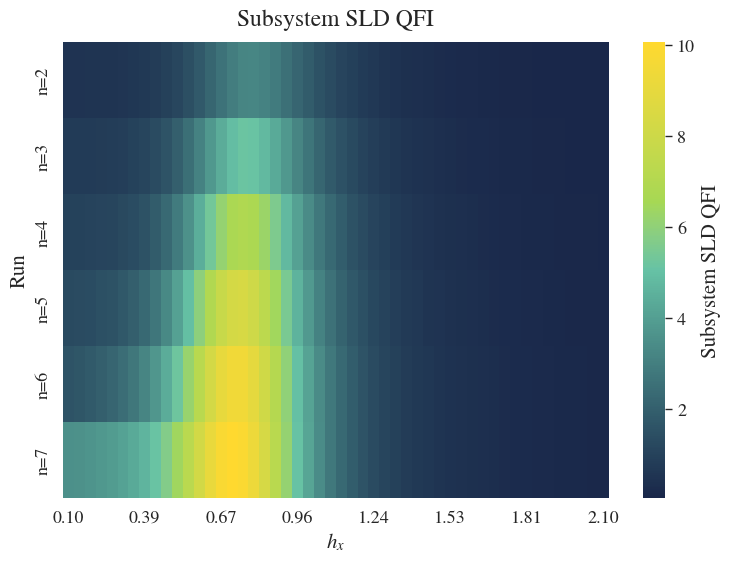
\includegraphics[width=0.48\textwidth]{figures/noise/project1/subsystem_SLD_varying_n_fixing_N8_heatmap.png}
    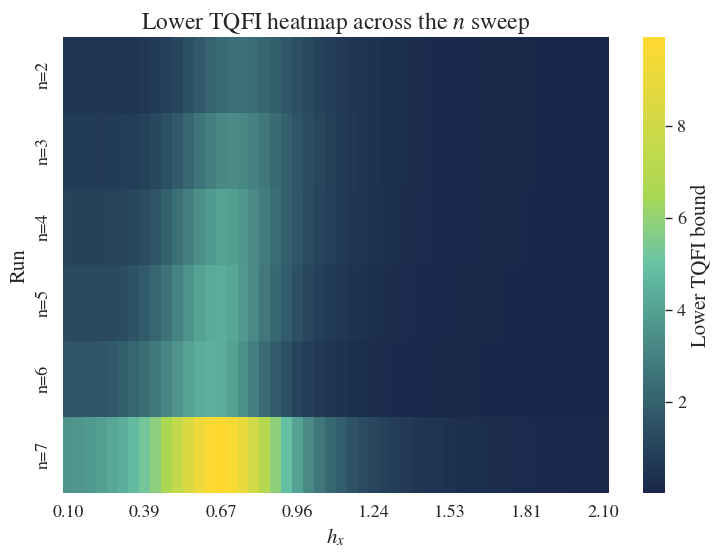
\includegraphics[width=0.48\textwidth]{figures/noise/project1/subsystem_TQFI_varying_n_fixing_N8_heatmap.png}

    \caption{Field-resolved exact local SLD QFI (left) and lower-TQFI diagnostic (right) as the accessible subsystem size increases at fixed $N=8$.}
    \label{fig:project1_fig_1_2_heatmaps}
\end{figure}


At the local-SLD peak, the lower-TQFI/SLD ratio ranges from about $0.42$ to $0.96$, and the corresponding sub-QFI/SLD ratio ranges from about $0.05$ to $0.60$. The finite-displacement quantities are informative but can be loose when the reduced state is strongly mixed. In the tested cases, the lower TQFI endpoint is closer to the exact SLD benchmark than the sub-QFI endpoint over the region of best recovery.

% ==============================================================================
\section{Global Thermal Preparation}
\label{sec:project7_noise}
% ==============================================================================

Temperature is introduced here at the preparation stage. For every value of $h_x$, the entire $N$-qubit probe is prepared in the Gibbs state $\rho_{\mathrm{th},N}(h_x;\beta)$ and only then reduced to the same accessible subsystem $S$. We keep $\beta$ fixed to define a parameterized thermal family and compare the local response at different inverse temperatures.

This calculation asks a practical question: as the global probe is cooled, how much of the field sensitivity of the low-temperature reference becomes accessible locally? The answer depends on both inverse temperature and the finite-size spectrum.

Related full-probe work has reported temperature-enhanced QFI in critical models~\cite{osterma2024}, lending context to the initially counterintuitive temperature-dependent behaviour found here.

The sampled inverse temperatures are
\[
    \beta=0.1,\ 0.25,\ 0.5,\ 1,\ 2,\ 5,\ 10,\ 25,\ 50.
\]
Larger $\beta$ corresponds to a colder Gibbs state. To summarize the recovery of the finite-displacement observable, we define $\beta_\star$ as the interpolated value at which the peak local \texttt{lower\_tqfi} reaches $90\%$ of the ground-state peak of the same quantity. This is a convenient operational marker: it says how cold the chosen finite system must be before this particular local proxy recovers most of its ground-state peak. It is not a critical inverse temperature and does not identify a thermodynamic phase transition.

\subsection{Temperature dependence in an open chain}

For $N=6$, $n=4$, and open boundaries:
\begin{table}[htbp]
    \centering
    \caption{Open-chain local recovery for $N=6$ and $n=4$. Each entry is the maximum over the scanned field interval. Peaks at different inverse temperatures need not occur at the same $h_x$.}
    \label{tab:project7_open_recovery}
    \begin{tabular}{c c c c}
        \toprule
        State        & Peak \texttt{lower\_tqfi} & Peak local SLD & Peak full SLD \\
        \midrule
        Ground state & $5.019$                   & $6.014$        & $6.782$       \\
        $\beta=1$    & $0.747$                   & $1.714$        & $2.730$       \\
        $\beta=2$    & $1.440$                   & $2.792$        & $4.292$       \\
        $\beta=5$    & $3.987$                   & $6.151$        & $9.578$       \\
        $\beta=10$   & $6.164$                   & $8.962$        & $16.916$      \\
        \bottomrule
    \end{tabular}
\end{table}

For this run, the ground-state \texttt{lower\_tqfi} peak is $5.019$, so the $90\%$ target used to define $\beta_\star$ is $4.517$. Interpolation gives $\beta_\star=6.216$. The table should be read as a comparison of the \emph{best sensing point} available at each inverse temperature, rather than a point-by-point comparison at one fixed field. As the Gibbs state is cooled, the local thermal response grows and its dominant feature moves from the edge of the scan towards the finite-size critical region (See Figure~\ref{fig:project7_tightness_heatmaps}).

At $\beta=10$, the peak local and full SLD values are larger than the corresponding ground-state peaks. This is not a fixed noisy channel undoing its own information loss. A fixed, parameter-independent channel would act on one already encoded family and could only reduce its QFI. Here the Gibbs state is prepared afresh for every $h_x$: changing $h_x$ changes both the eigenvectors and the thermal populations. The thermal and ground-state rows are consequently different parameterized families, with no universal ordering of their peak QFIs.

\begin{infobox}{Why can a thermal peak exceed a ground-state peak?}
    Changing the field has two effects on a Gibbs state. First, it changes the Hamiltonian eigenvectors, just as for the ground state. Second, it changes the energies and hence the Boltzmann populations of the low-lying levels. At finite temperature, both effects can carry information about $h_x$.

    The second effect is particularly important near a small gap. Around the open-chain feature at $h_x=0.547$, the first excitation gap is approximately $\Delta=0.038$. Even at $\beta=50$, the relative Boltzmann weight of that excitation is $e^{-\beta\Delta}\approx e^{-1.9}\approx0.15$, so it is not negligible there. A small field variation can then significantly redistribute population between the low-energy levels, enhancing the thermal QFI at that field.

    At any fixed field with a nondegenerate ground state, the Gibbs state approaches the ground state as $\beta\rightarrow\infty$. The apparent enhancement in Table~\ref{tab:project7_open_recovery} instead concerns maxima over a finite field window: at each $\beta$, the maximization can select the field with the most responsive low-energy spectrum. It is a finite-size spectral effect, not a statement that finite temperature is always beneficial or that the thermal family has more QFI at every fixed field.
\end{infobox}


% \begin{figure}[H]%[htbp]
%     \centering
%     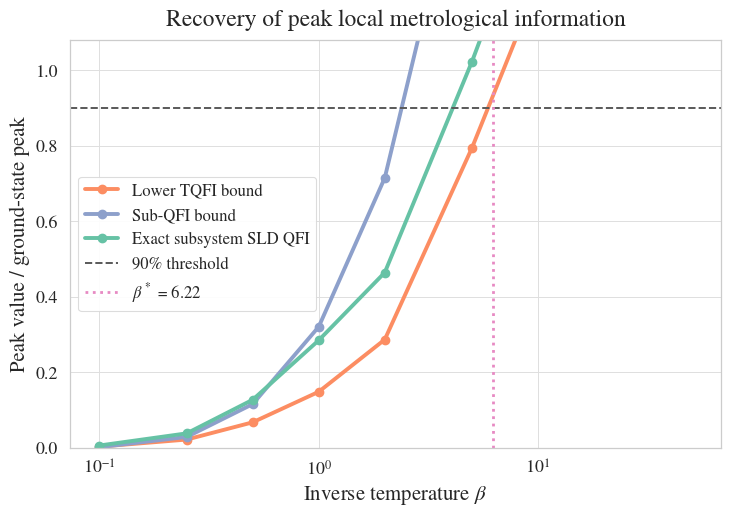
\includegraphics[width=1\textwidth]{figures/noise/project7/recovery_peak_vs_beta.png}
%     \caption{Recovery of the peak local information as the inverse temperature $\beta$ increases for the open $N=6$, $n=4$ chain.}
%     \label{fig:project7_fig_7_1}
% \end{figure}

% \todo[]{insert diagram 9}

% \noindent\emph{Plot brief.} Insert Project~7 figure P7.2: ground-state local bounds and local SLD with the thermal \texttt{lower\_tqfi} overlay, showing peak migration.

\begin{figure}[H]%[htbp]
    \centering
    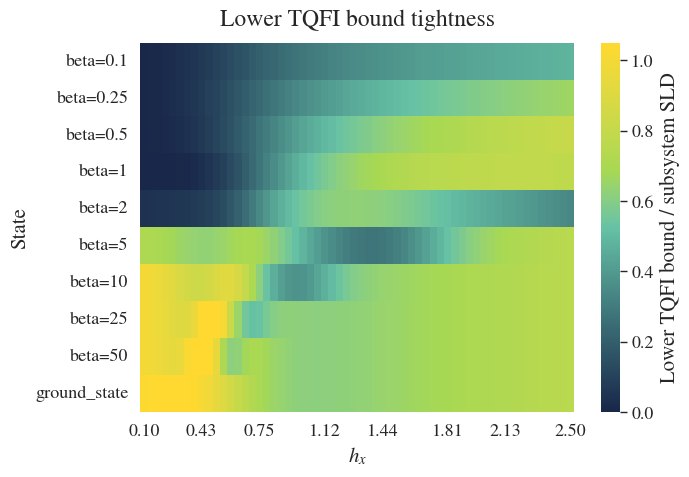
\includegraphics[width=0.48\textwidth]{figures/noise/project7/heatmap_proj7_TQFI_tight.png}
    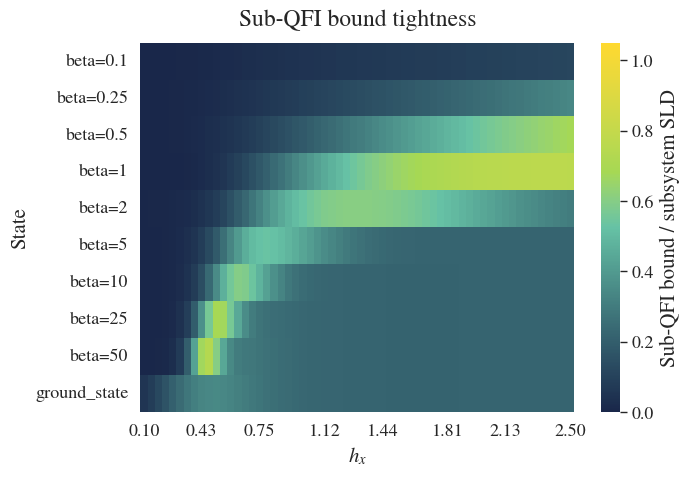
\includegraphics[width=0.48\textwidth]{figures/noise/project7/heatmap_proj7_subQFI_tight.png}
    \caption{Tightness of the lower TQFI endpoint (left) and sub-QFI endpoint (right) relative to the exact local SLD benchmark across inverse temperature $\beta$.}
    \label{fig:project7_tightness_heatmaps}
\end{figure}

% ==============================================================================
\section{Comparing the Three Preparation Histories}
\label{sec:project9_noise}
% ==============================================================================

This is the main controlled comparison.  It places $\rho_{\mathrm{G},S}$, $\rho_{\mathrm{dep},S}$, and $\rho_{\mathrm{th},S}$ on  an equal number $n$ of qubits. The observer retains the same size subsystem while the full probe is prepared in different ways. Local QFI is the primary output. The fixed-control data satisfy the consistency checks in Eqs.~\eqref{eq:depolarizing_data_processing} and~\eqref{eq:local_global_data_processing}. For the field-by-field matched-purity paths, $P$ and $\beta$ depend on $h_x$, so the fixed-channel ordering relative to the ground family does not apply, only the full-to-local inequality within each matched family remains required.

The four comparisons answer different questions:
\begin{itemize}
    \item the first tests whether matching purity makes distinct local state families metrologically equivalent,
    \item the second asks how the three local families change as access to the probe grows,
    \item the third isolates the fixed depolarizing channel,
    \item the fourth is the central inverse-temperature sweep of the globally Gibbs-prepared family.
\end{itemize}

\subsection{Matched purity regime}
\label{sec:project10_peak_purity}

We use the matched-purity construction to test whether equal purity alone can make distinct local state families metrologically equivalent.

\paragraph{Field-by-field matched-purity diagnostic.}
Almost zero depolarization and a very cold Gibbs state can match each other and the reduced ground-state subsystem in the near-pure limit. This is a useful numerical consistency check, but it is too close to the ground-state limit to isolate the role of purity.

The non-trivial version retains $n=5$ qubits of an open $N=6$ chain and uses
the purity of a further reduced ground-state $n=4$ state as the target.  The
globally depolarized and globally Gibbs-prepared $n=5$ states match that target
at every sampled field\footnote{The absolute purity-matching residuals are below $10^{-8}$.}. Their local QFI
curves still differ.  This is the basic result: equal purity does not make the
two local state families metrologically equivalent.

In this field-by-field construction, however, both $P$ and $\beta$ are
retuned as $h_x$ changes.  It is therefore best read as a clean test of the
role of purity, not as the performance of one fixed sensor.  In particular,
very steep changes in the matched inverse temperature can strongly affect the
derivative used in the QFI.

The numerical QFI for these matched paths includes the total-derivative terms; the branch-specific expressions are given in Appendix~\ref{app:matched_purity_derivatives}.

\paragraph{Fixed-control comparison.}
For the experimentally more direct comparison, we keep $P$ or $\beta$ fixed
throughout each field scan and then find the best local-SLD peak.  The left
panel of Figure~\ref{fig:project10_peak_purity} compares the peak QFI with the
purity at that same peak, $\gamma_\star=\operatorname{Tr}[\rho_S^2(h_x^\star)]$. At a given horizontal position, the higher point
corresponds to the family with the better peak sensitivity.  The ordering
changes: near $\gamma_\star=0.439$, the $\beta=2$ thermal peak is lower than
the depolarized one, $3.531$ versus $5.167$, while near
$\gamma_\star=0.586$, the $\beta=5$ thermal peak is higher, $7.938$ versus
$6.157$.  At $\beta=50$, a similar peak purity gives a peak QFI of $16.342$,
compared with $6.139$ for the depolarized reference.

The right panel shows that purity also does not select a unique operating
field.  The depolarized peaks remain close to $h_x^\star=0.62$, whereas the
thermal peaks move over the sampled range.  The conclusion is limited to this
finite system and these controls: thermal preparation is not always better,
but purity by itself does not determine either the best local QFI or where the
best operating point lies.

\begin{figure}[H]
    \centering
    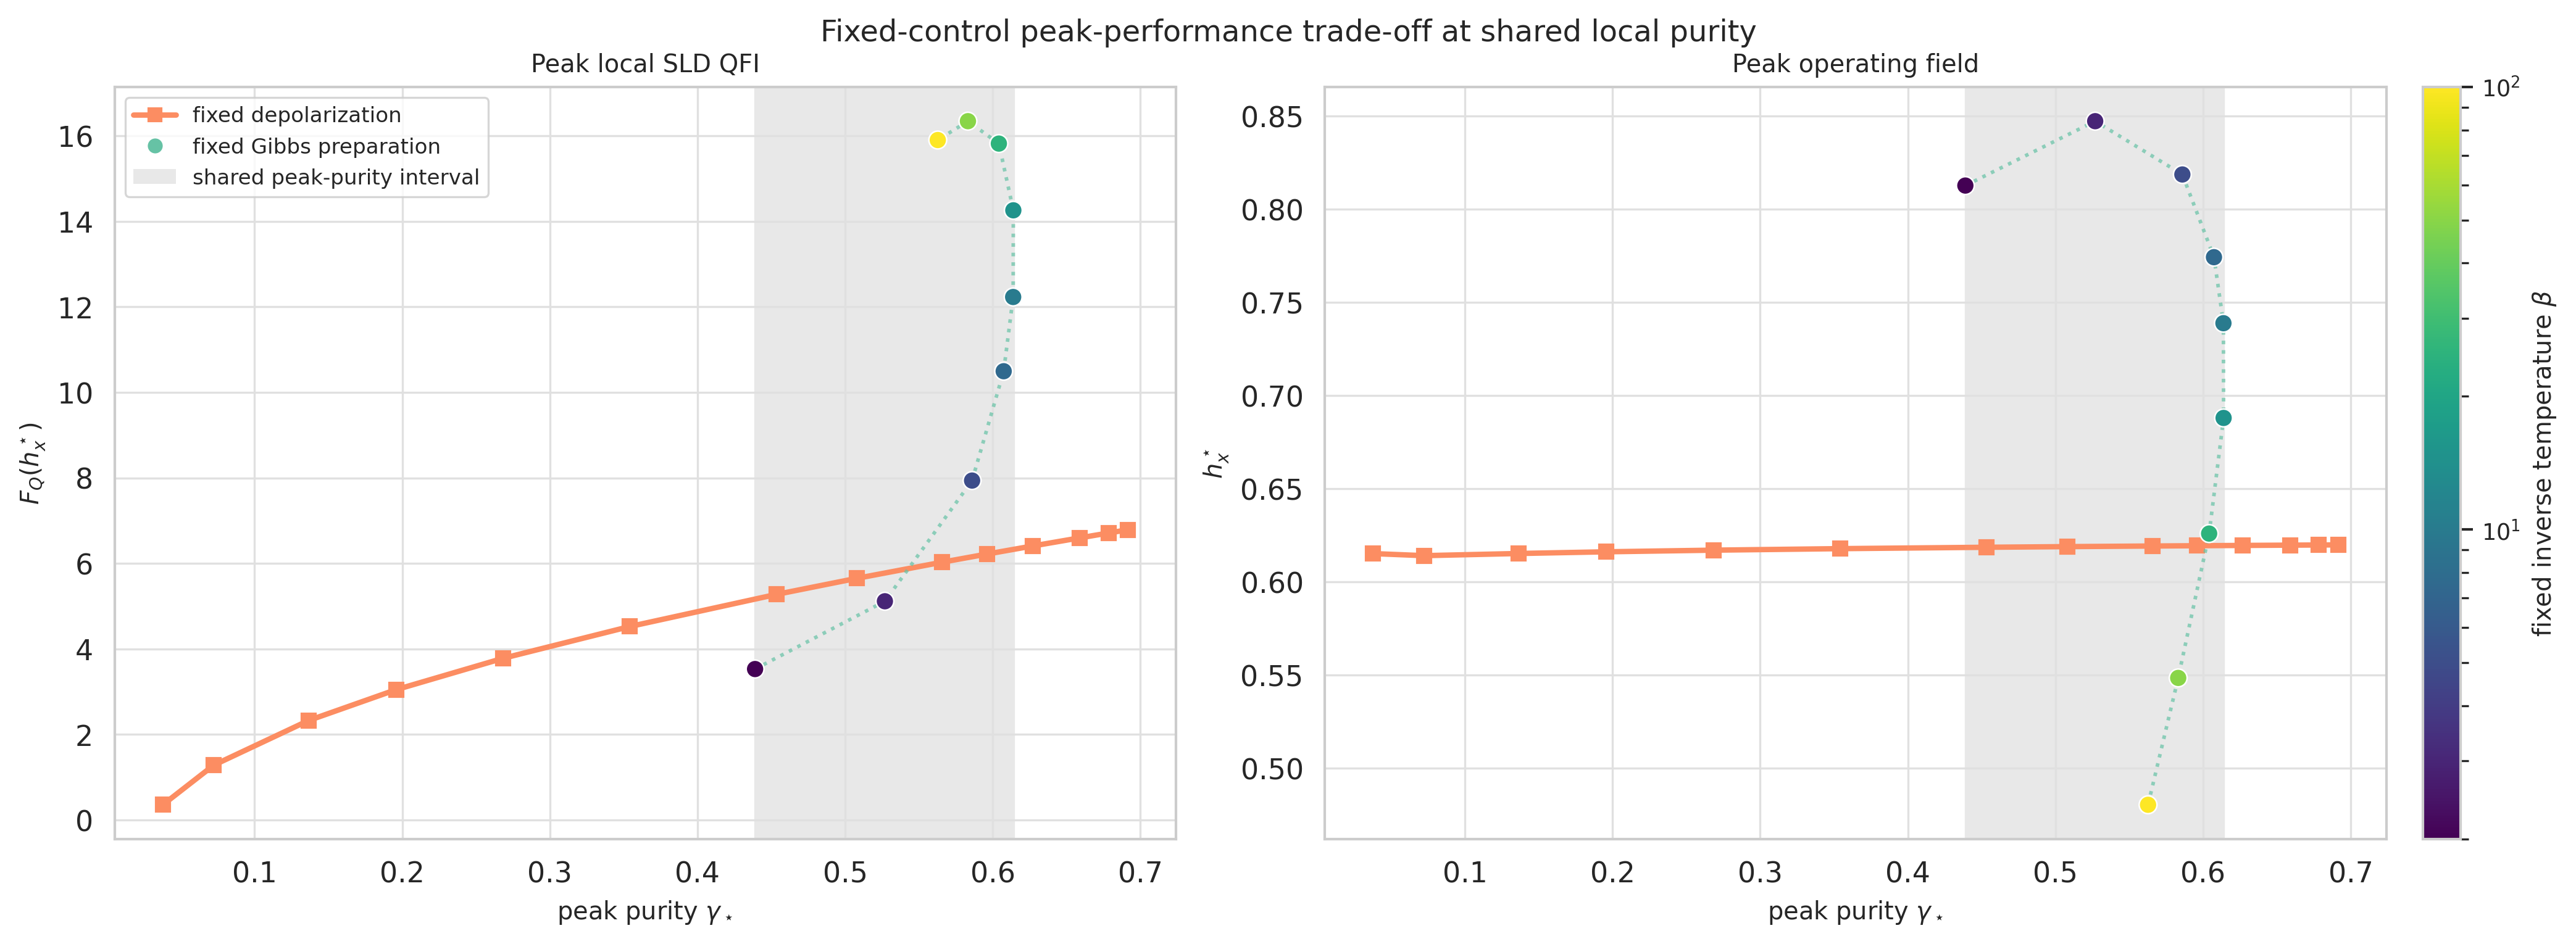
\includegraphics[width=\textwidth]{figures/noise/project9/project10_fixed_control_peak_purity.png}
    \caption{Fixed-control peak comparison for the open $N=6$, $n=5$ chain.
        Each orange square is one fixed depolarizing probability $P$; each coloured
        circle is one fixed inverse temperature $\beta$.  Left: peak local SLD QFI
        versus the purity at that peak.  At the same horizontal position, the
        higher point has the larger peak sensitivity.  Right: the field at which
        the same peak occurs.  The shaded region is the range of peak purities
        sampled by both families; the dotted thermal line is only a guide between
        the sampled temperatures. It is more clear if one follows the line of the thermal points on inverse temperature, from the hotter (bluer) to the cooler (more yellow). There we can notice their purity and informativity changes while cooling down.}
    \label{fig:project10_peak_purity}
\end{figure}


\subsection{Accessible subsystem size}

For $N=6$ with periodic boundaries:
\begin{table}[htbp]
    \centering
    \caption{Local SLD-QFI peaks versus accessible subsystem size at fixed preparation controls. The full $N=6$ ground-state reference has peak QFI $4.344$ over the same grid.}
    \label{tab:project9_preset_b}
    \begin{tabular}{c c c c}
        \toprule
        $n$ & $\rho_{\mathrm{G},S}$ & $\rho_{\mathrm{dep},S}$ & $\rho_{\mathrm{th},S}$ \\
        \midrule
        $1$ & $0.972$               & $0.722$                 & $0.348$                \\
        $2$ & $2.134$               & $1.724$                 & $0.688$                \\
        $3$ & $3.164$               & $2.672$                 & $1.040$                \\
        $4$ & $3.926$               & $3.419$                 & $1.393$                \\
        $5$ & $4.344$               & $3.865$                 & $1.741$                \\
        \bottomrule
    \end{tabular}
\end{table}

At the principal peak in this $\beta=1$ baseline,
\[
    \mathcal{F}_Q[\rho_{\mathrm{G},S}]\geq
    \mathcal{F}_Q[\rho_{\mathrm{dep},S}]>
    \mathcal{F}_Q[\rho_{\mathrm{th},S}]
\]
Peak ordering is not the full field-resolved story.  In every $n$ run, the thermal family exceeds the reduced ground-state family over broad off-peak intervals. For $n=4$, the largest pointwise thermal advantage is $0.456$ at $h_x=1.686$.

\faLightbulb \hspace{5pt} An important fact is that a state family can be inferior by maximum QFI while being superior over a useful interval of the operating field, which is why the chapter reports both peak tables and field-resolved plots.

% \todo[]{insert diagram 13}

% \noindent\emph{Plot brief.} Insert Project~9 figure P9.1: peak local SLD QFI versus $n$ for the three local families.

\subsection{Depolarizing strength}

For $N=6$, $n=4$, periodic boundaries, and varying only $P$:
\begin{table}[htbp]
    \centering
    \caption{Peak local SLD QFI under the fixed full-system depolarizing channel in Eq.~\eqref{eq:full_depolarizing_channel}.}
    \label{tab:project9_preset_d}
    \begin{tabular}{c c c}
        \toprule
        $P$    & Peak $\mathcal{F}_Q[\rho_{\mathrm{dep},S}]$ & Change from $P=0$ \\
        \midrule
        $0.00$ & $3.926$                                     & $0\%$             \\
        $0.05$ & $3.661$                                     & $-6.7\%$          \\
        $0.10$ & $3.419$                                     & $-12.9\%$         \\
        $0.20$ & $2.953$                                     & $-24.8\%$         \\
        $0.30$ & $2.499$                                     & $-36.4\%$         \\
        \bottomrule
    \end{tabular}
\end{table}

Depolarization lowers local QFI smoothly and monotonically.  The ground-subsystem and thermal curves remain unchanged in this sweep because only $P$ is varied.

\begin{figure}[H]
    \centering
    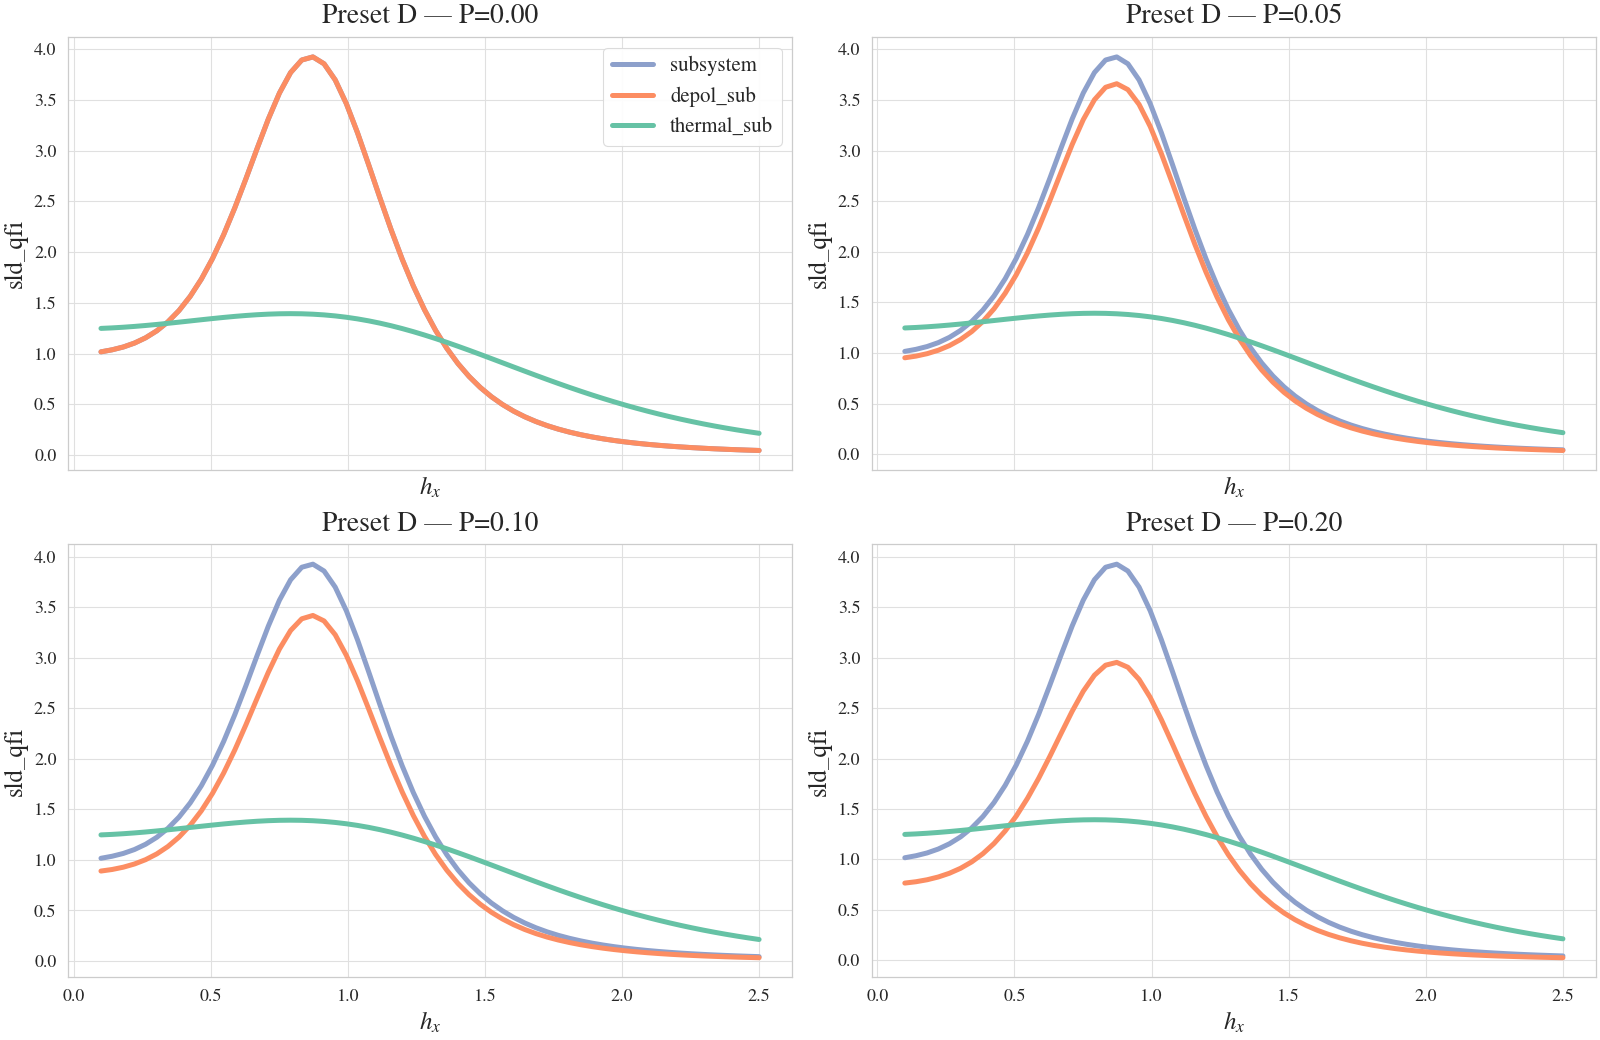
\includegraphics[width=\textwidth]{figures/noise/project9/polarization_comparison.png}
    \caption{Field-resolved local SLD QFI for several fixed depolarizing probabilities $P$.}
    \label{localqfi_vs_depolarizing}
\end{figure}

\begin{figure}[H]
    \centering
    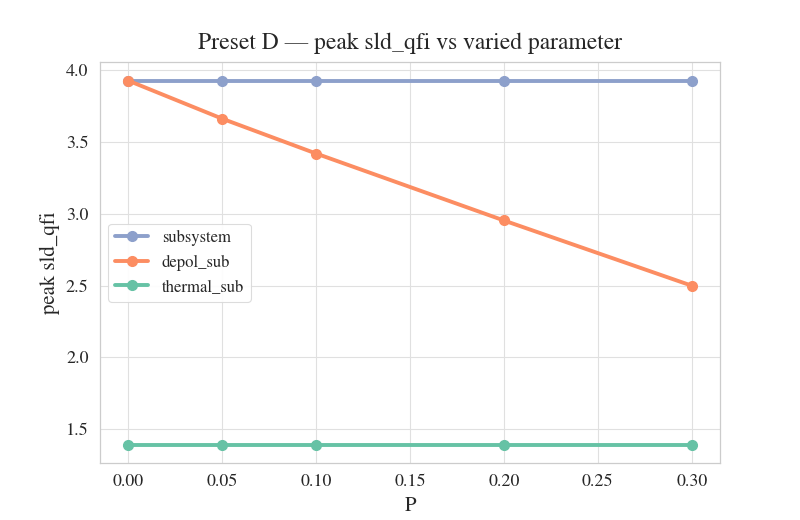
\includegraphics[width=0.7\textwidth]{figures/noise/project9/polarization_evolution.png}
    \caption{Peak local SLD QFI versus depolarizing probability $P$.}
    \label{localqfi_vs_depolarizing_evo}
\end{figure}


\subsection{Temperature sweep at fixed accessible size}

For $N=6$, $n=4$, and periodic boundaries, the depolarized comparator uses fixed $P=0.1$ while the thermal branch varies $\beta$:
\begin{table}[htbp]
    \centering
    \caption{Thermal inverse-temperature sweep at fixed accessible size. The ground-subsystem peak is $3.926$, and each thermal entry is the maximum over the field grid.}
    \label{tab:project9_preset_e}
    \begin{tabular}{c c c c}
        \toprule
        $\beta$ & Peak $\mathcal{F}_Q[\rho_{\mathrm{th},S}]$ & Peak field & Relation to ground subsystem             \\
        \midrule
        $0.2$   & $0.152$                                    & $0.100$    & strongly suppressed                      \\
        $0.5$   & $0.729$                                    & $0.100$    & suppressed                               \\
        $1.0$   & $1.393$                                    & $0.792$    & suppressed                               \\
        $2.0$   & $2.607$                                    & $1.076$    & lower peak, pointwise crossings occur    \\
        $5.0$   & $4.847$                                    & $1.036$    & $23.5\%$ above the ground-subsystem peak \\
        \bottomrule
    \end{tabular}
\end{table}

At $\beta=5$, the thermal local QFI is greater than the reduced-ground-state local QFI at $40/60$ sampled fields. It remains bounded by its full thermal parent:
\begin{equation}
    \max_{h_x}\mathcal{F}_Q[\rho_{\mathrm{th},S}]
    =4.847
    <
    8.456
    =\max_{h_x}\mathcal{F}_Q[\rho_{\mathrm{th},N}]
    \label{eq:project9_thermal_consistency}
\end{equation}

The finite-system mechanism is the field dependence of low-lying thermal populations, not an increase of QFI under a fixed channel.

For the finite TFIM geometries and field windows studied here, thermal preparation before partial trace can enhance local SLD QFI relative to the reduced ground-state subsystem.  The effect depends on the regime, is strongest at larger $\beta$ in the present sweep, and remains bounded by the QFI of the full thermal family.



\begin{figure}[H]
    \centering
    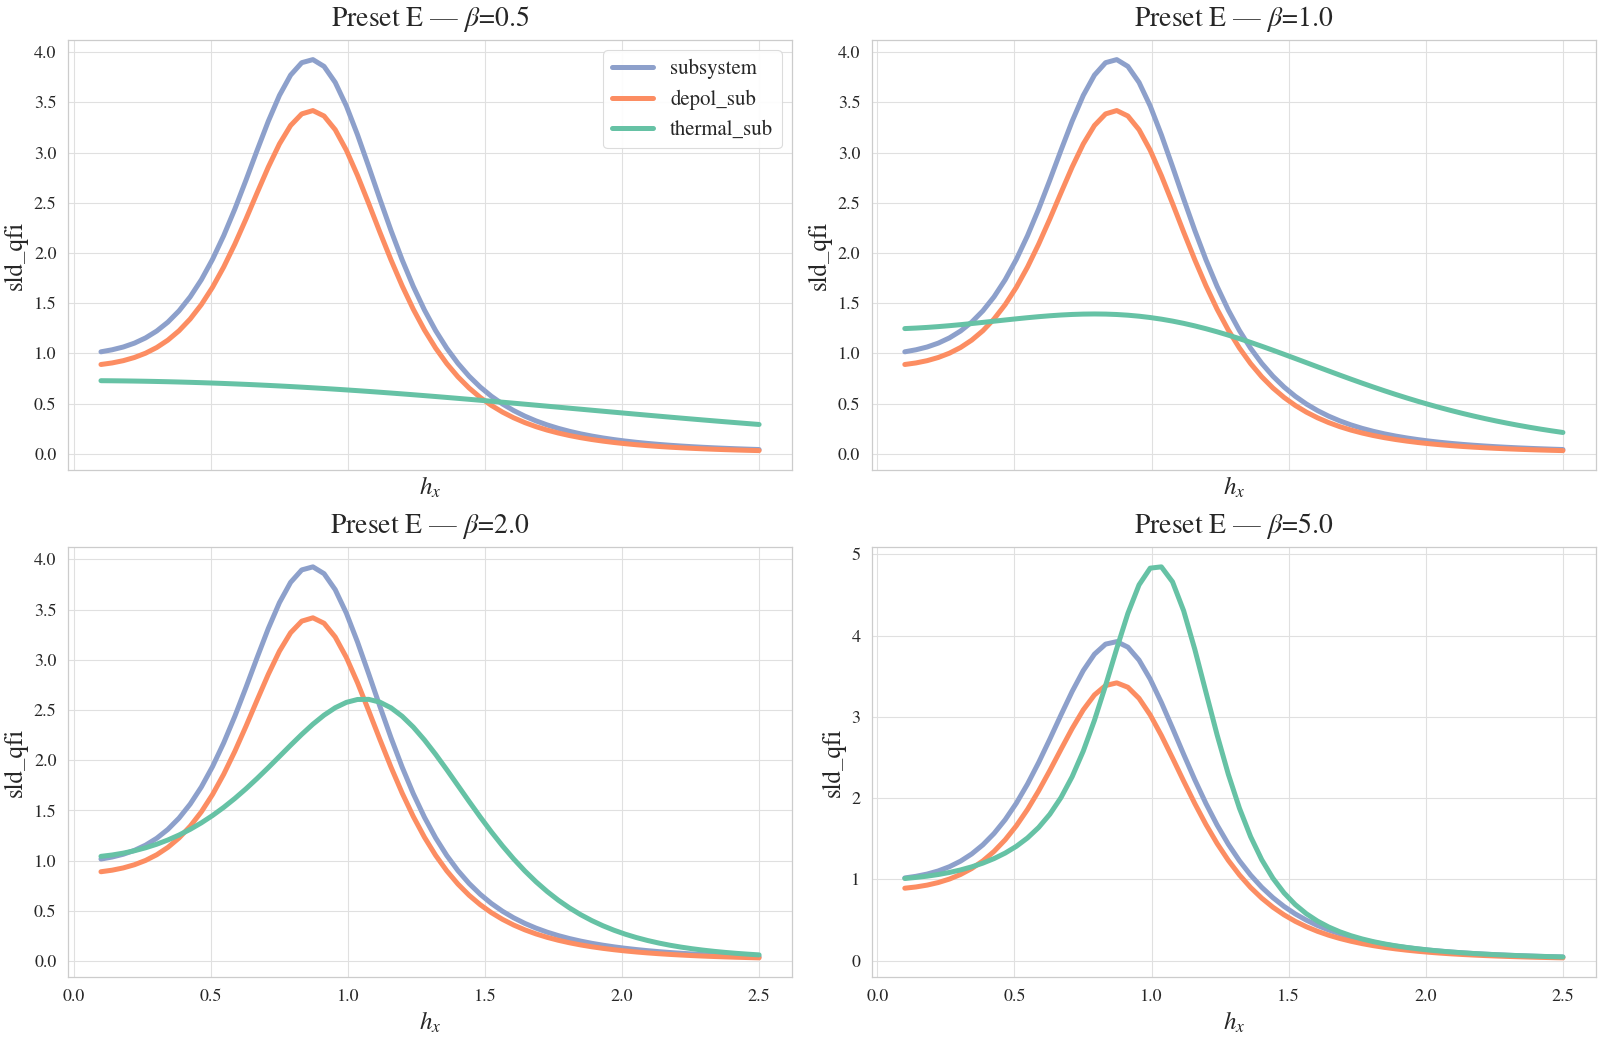
\includegraphics[width=\textwidth]{figures/noise/project9/thermal_comparison.png}
    \caption{Field-resolved local SLD QFI for several fixed inverse temperatures $\beta$.}
    \label{localqfi_vs_thermal}
\end{figure}


\begin{figure}[H]
    \centering
    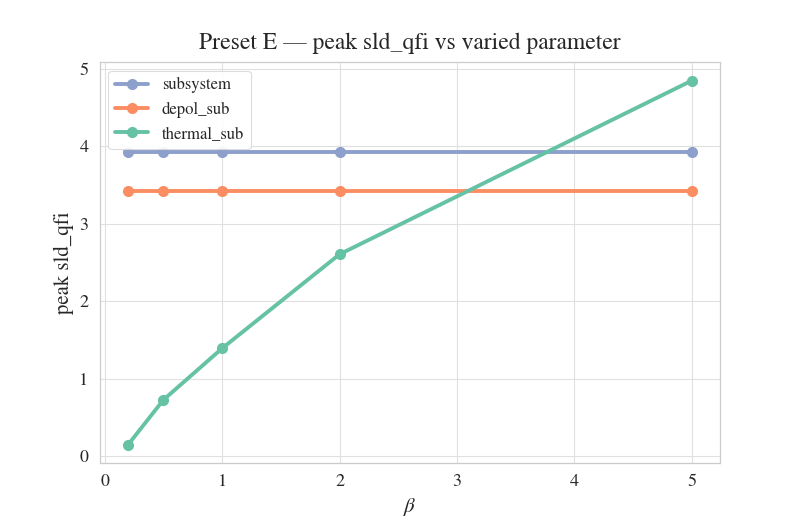
\includegraphics[width=0.7\textwidth]{figures/noise/project9/thermal_evolution.png}
    \caption{Peak local SLD QFI versus inverse temperature $\beta$.}
    \label{localqfi_vs_thermal_evo}
\end{figure}


% ==============================================================================
\section{Conclusions}
\label{sec:noise_synthesis}
% ==============================================================================



Critical metrological response is spatially distributed.  Partial trace removes a variable fraction of it, and the retained fraction grows strongly with accessible subsystem size.

Entanglement-induced mixedness, depolarization, and thermal population are not interchangeable.  Purity alone does not predict local QFI: the field dependence of the state and the part of the spectrum populated by the preparation both matter.

% \subsection{What these results do not establish}

% The present data do not support a universal QFI scaling exponent.  Thermal preparation is not generically beneficial and should never be described as a fixed channel increasing QFI of the same encoded family.  Local TQFI should not be compared directly with global SLD QFI, and lower TQFI should not be called a strict pointwise SLD lower bound at the present finite displacements.


% \subsection{A methodological lesson}

% Exact local SLD QFI is the correct benchmark where it can be computed.  Finite-displacement TQFI adds a complementary operational layer by testing whether a truncated or fidelity-based description retains the same feature.  It should be validated against exact local SLD on small systems before it is used where exact SLD is unavailable.

% \subsection{Limitations and outlook}

% The present data establish finite-system trends rather than asymptotic laws.  A controlled size study, performed separately at fixed accessible size $n$ and fixed retained fraction $n/N$, is required before assigning scaling exponents to peak heights or locations.  The low-temperature limit should likewise be checked through pointwise convergence of the thermal family to the reduced ground-state family and through more than one well-defined crossover diagnostic.

For the finite probes studied here, local metrological performance depends on the full sequence that produces the accessible state.  Access to the relevant subsystem, the low-energy spectrum, and the way mixedness is prepared all matter.

